\section{Отсечение невидимых поверхностей. Z-буфер и алгоритм художника.}


\textbf{Задача:}\\
Дана сцена с 2D или 3D объектами и наблюдатель, который смотрит на сцену из своей точки обзора. 
Нужно отрисовать на сцене видимые наблюдателю части объектов.

\subsection{Алгоритм z-буфера (z-buffer algorithm)}

Для \textbf{отсечения невидимых частей поверхности} существует простой, но длительный метод — алгоритм z-буфера. В направлении просмотра проводится ось z-координат, затем определяется, какие пиксели покрывают проекции объектов. Алгоритм хранит информацию об уже обработанных объектах в двух буферах: буфере кадра и z-буфере.

\begin{itemize}
	\item В буфере кадра для каждого пикселя хранится информация о цвете объекта, отображаемого им на данный момент.
	\item В z-буфере для каждого пикселя хранится z-координата видимого на данный момент объекта, точнее, в нем хранится z-координату точки такого объекта.
\end{itemize}

Предположим, что мы выбрали пиксель и преобразовываем объект.

\begin{itemize}
	\item Если z-координата объекта в этом пикселе меньше, чем z-координата, хранимая в z-буфере, тогда новый объект лежит перед видимым на данный момент (меняем z-буффер и буфер кадра) 
	\item Если z-координата объекта в этом пикселе больше, чем z-координата, хранимая в z-буфере, то новый объект не видим, и буферы останутся без изменений.
\end{itemize}
Алгоритм z-буфера легко реализовать, и он быстро работает, но требует много дополнительной памяти
\newpage
\subsection*{Алгоритм художника (painter's algorithm)}

Алгоритм художника избегает дополнительных затрат памяти, изначально сортируя объекты по расстоянию от них до точки обзора. 
Тогда объекты проверяются в \textbf{порядке глубины}, начиная от самого дальнего.

\begin{figure}[h!]
	\centering
	
\includegraphics[width=0.4\linewidth]{img/16_1.png}
	\captionsetup{labelformat=empty}
	\caption{Пример работы алгоритма художника}
\end{figure}


\textbf{Основная проблема}: порядок глубины не всегда существует: отношение "перед" может содержать циклы. Когда такое цикличное перекрытие происходит, объекты не могут быть корректно отсортированы. 

\begin{figure}[h!]
	\centering
	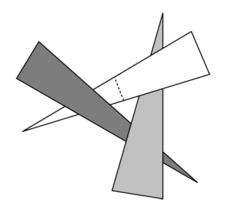
\includegraphics[width=0.4\linewidth]{img/16_2.png}
	\captionsetup{labelformat=empty}
	\caption{Иллюстрация циклического наложения фигур --- проблемы данного алгоритма}
\end{figure}

\textbf{Решение:} сортировка фрагментов объектов (сначала --- разбиение объектов на фрагменты)

Задачу разбиение на фрагменты можно решить с помощью \textbf{двоичного разбиения пространства} (англ. binary space partitioning, BSP)

\newpage
\subsection{BSP-деревья}

Покажем двоичное разбиение пространства на примере рисунка ниже

\begin{figure}[h!]
	\centering
	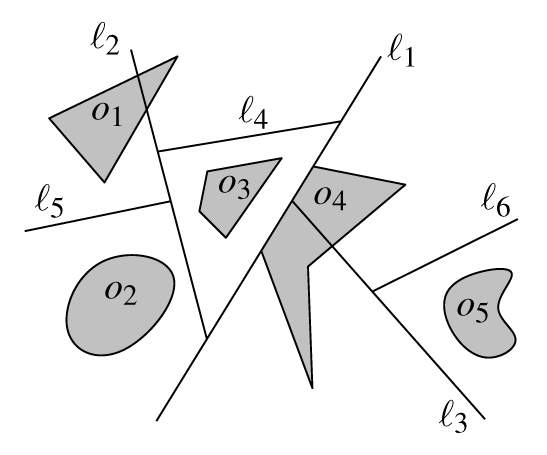
\includegraphics[width=0.4\linewidth]{img/16_3.png}
	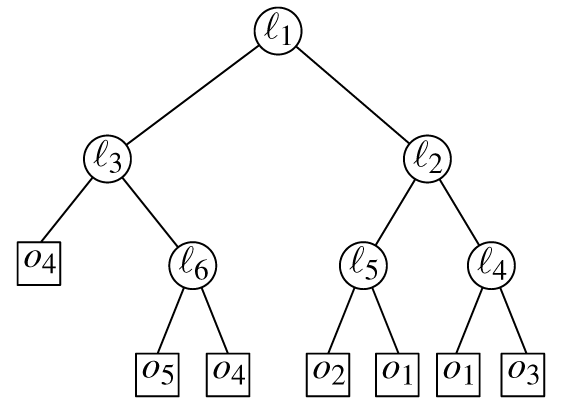
\includegraphics[width=0.4\linewidth]{img/16_4.png}
	\captionsetup{labelformat=empty}
	\caption{}
\end{figure}

Прямые разбивают на части не только плоскость, но и объекты, расположенные на ней. Разбиение продолжается до тех пор, пока внутри каждой грани плоскости окажется не более одного фрагмента объекта.

Этот процесс можно представить с помощью двоичного дерева. Каждый лист дерева соответствует \textbf{грани разбиения}, в нем хранится фрагмент объекта, находящийся внутри этой грани. 
Каждый узел дерева соответствует \textbf{разбивающей прямой}, которая хранится в этом узле.

\begin{definition}
	\textbf{BSP-дерево} (англ. binary space partition tree) — дерево, отвечающее заданному двоичному разбиению пространства.
\end{definition}

\textbf{Свойства BSP-деревьев}

Пусть гиперплоскость h делит пространство на h+ и h-
Пусть $S$ — множество объектов, для которого мы строим разбиение в $d$-мерном пространстве, $v$ — какая-то вершина дерева, тогда
обозначим за $S(v)$ множество объектов (возможно пустое), хранимых в этой вершине.
\begin{itemize}
	\item Если $|S| \leq1$, то T — лист. Фрагмент объекта в S , если он существует, хранится в этом листе.
	\item Если $|S| > 1$ , то в корне дерева $v$ хранится гиперплоскость h и множество $S(v)$ объектов, которые полностью содержатся в h.
	
\end{itemize}
\subsection*{BSP-деревья и алгоритм художника}

Предположим, что мы построили BSP-дерево T
для множества объектов S в трехмерном пространстве. 

Пусть $p_{view}$
— точка обзора, и она лежит над разбивающей плоскостью, хранимой в корне T.

Тогда ни один из объектов, лежащих под этой плоскостью, не может перекрыть ни один из объектов, лежащих выше нее. 
Таким образом, мы можем безопасно отрисовать фрагменты объектов из поддерева $T^-$ до отрисовки объектов из поддерва $T^+$. 
Порядок фрагментов объектов в поддеревьях определяется таким же способом.


